\documentclass[border=4pt]{standalone}

% --- packages (mirror these in layer.meta.json "requires") ---
\usepackage{tikz}

% --- palette (canonical source: reference/color-palettes/color-palettes.md; light variant) ---
\definecolor{otblue}{HTML}{0072B2}
\definecolor{otorange}{HTML}{E69F00}
\definecolor{otteal}{HTML}{009E73}
\definecolor{otpurple}{HTML}{CC79A7}
\definecolor{otgray}{HTML}{5A5A5A}

\begin{document}
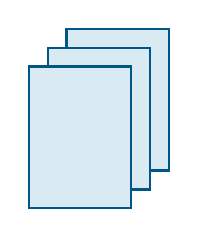
\begin{tikzpicture}[line width=0.8pt]
  % stacked feature maps (back to front for correct overlap)
  \foreach \i in {2,1,0}{
    \pgfmathsetmacro{\d}{\i*0.24}
    \filldraw[draw=otblue!75!black, fill=otblue!15] (\d,\d) rectangle (\d+1.3,\d+1.8);
  }
\end{tikzpicture}
\end{document}
